 % !TeX program = lualatex
% !TeX encoding = utf8
% !TeX spellcheck = uk_UA
% !BIB program = bibtex8

\documentclass[]{article}

\usepackage{fontspec}
\setsansfont{CMU Sans Serif}%{Arial}
\setmainfont{CMU Serif}%{Times New Roman}
\setmonofont{CMU Typewriter Text}%{Consolas}
\defaultfontfeatures{Ligatures={TeX}}
\usepackage[math-style=TeX]{unicode-math}
\usepackage[english, russian, ukrainian]{babel}
\usepackage[%
	a4paper,%
	footskip=1cm,%
	headsep=0.3cm,% 
	top=1cm, %поле сверху
	bottom=1cm, %поле снизу
	left=1cm, %поле ліворуч
	right=1cm, %поле праворуч
    ]{geometry}

\usepackage{tikz}
\usetikzlibrary{shadows}
\usepackage[many, most]{tcolorbox}
\newtcolorbox{tornpage}{%
    enhanced jigsaw, % allow page breaks
    frame hidden, % hide the default frame
    overlay={%
        \draw [
            fill=white, % fill paper
            draw=white!50!black, % boundary colour
            decorate, % decoration
            decoration={random steps,segment length=2pt,amplitude=1pt},
            drop shadow, % shadow
        ]
        % top line
        (frame.north west)--(frame.north east)--
        % right line
        (frame.north east)--(frame.south east)--
        % bottom line
        (frame.south east)--(frame.south west)--
        % left line
        (frame.south west)--(frame.north west);
    },
    % paragraph skips obeyed within tcolorbox
    parbox=false,
}
\usepackage{caption}
\usepackage{booktabs}
\usepackage{pgfplots, pgfplotstable}
\usetikzlibrary{fpu}
\usetikzlibrary{intersections}
\usetikzlibrary{backgrounds}
\usetikzlibrary{arrows.meta}  
\usetikzlibrary{intersections}
\usepackage{graphicx}

\pgfkeys{/pgf/number format/.cd,custom exponent/.initial=2}%
\newcommand{\pgfmathprintnumberFE}[2][]{%
\begingroup
\pgfkeys{/pgf/number format/.cd,fixed,#1}%
\pgfset{fpu=true}%
\pgfmathparse{#2}%
\pgfmathfloattomacro{\pgfmathresult}{\F}{\M}{\E}%
\pgfset{fpu=false}%
\pgfmathtruncatemacro{\redexp}{\E-\pgfkeysvalueof{/pgf/number format/custom exponent}}%
\ifnum\pgfkeysvalueof{/pgf/number format/custom exponent}=0
\ensuremath{\pgfmathprintnumber[#1]{\pgfmathresult}}%
\else
\pgfmathsetmacro{\newnum}{\M*pow(10,\redexp)}%
\ensuremath{\pgfmathprintnumber{\newnum}\cdot10^{\pgfkeysvalueof{/pgf/number format/custom exponent}}}%
\fi
\endgroup}

\newcommand\GetMean[2]{
  \pgfplotstableread{#1}\tableA
  \pgfplotstableset{
    create on use/new/.style={
    create col/expr={\pgfmathaccuma + \thisrow{#2}}},
  }
  \pgfplotstablegetrowsof{\tableA}
  \pgfmathsetmacro{\NumRows}{\pgfplotsretval}
  \pgfplotstablegetelem{\numexpr\NumRows-1\relax}{new}\of{#1} 
  \pgfmathsetmacro{\Sum}{\pgfplotsretval}
  \pgfmathsetmacro{\Mean}{\Sum/\NumRows}
}

\begin{document}
\begin{center}
Звіт з лабораторної роботи \textnumero 5.3\\
\bigskip
{\large\bfseries Вивчення інтерференції світла при відбиванні від товстої скляної пластини}
\end{center}
\begin{center}
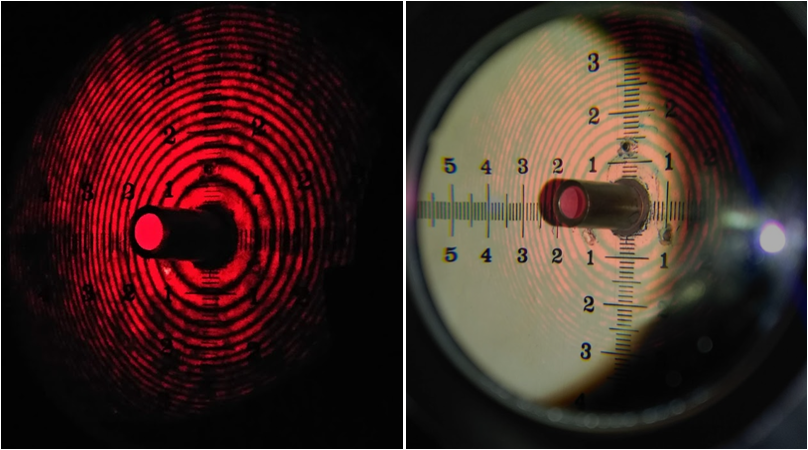
\includegraphics[width=0.95\linewidth]{L=61}
\label{fig:L=61}
\end{center}

\pagestyle{empty}

%========================================== Завантаження данних з таблиці ===================================================%
%----- Присвоєння данних змінній \TorqueVsCurrentTable
\pgfplotstableread{measured.dat}\ExpTable



%========================================== Додавання нової колонки в таблицю =============================================%
%----- Додається нова колонка 

\pgfplotstablecreatecol[
	create col/expr={\thisrow{r}^2},
]{rsqr}\ExpTable

\pgfplotstablecreatecol[
	create col/expr={\thisrow{rError}^2},
]{rsqrError}\ExpTable

%---------------------------------------------------------

\begin{center}
	\begin{tikzpicture}[
			declare function={
					L  = 61-2;
					lambda  = 6.3285e-5;
					d  = 1.625;	
				},
		]


		\begin{axis}[
				% === Налаштування сітки ===
				grid = both,
				major grid style={line width=.6pt,draw=brown!60},
				minor tick num = 9,
				minor grid style = {line width=.1pt,draw=brown!20},
				% === Налаштування положення координатних осей ===
				axis lines = middle,
				axis line style={-stealth},
				% === Підпис координатних осей ===
				%				xticklabels={},
				xlabel={$N$},
				ylabel={$r^2$, см$^2$},
				% === Положення підпису координатних осей ===
				ylabel style={above right},
				every tick/.style={black},
%				extra tick style={% changes for all extra ticks
%						tick align=outside,
%						major grid style={dashed,draw=black}
%					},
%			    extra x tick style={
%			      red,
%			      major tick style={
%			        gray,
%			      },
%			      tick label style={
%					yshift=6mm,
%			        /pgf/number format/.cd, fixed, fixed zerofill,
%			        precision=2,
%			      }
%			    },
%				extra y tick style={% changes for extra y ticks
%						tick label style={yshift=2mm},
%					},
				extra x ticks={2, 3, 4, 5, 6},
%				extra x tick labels={
%					\pgfmathprintnumberFE[custom exponent=0]{F1(1/sqrt(2))/100},
%					\pgfmathprintnumberFE[custom exponent=0]{nures/100},
%					\pgfmathprintnumberFE[custom exponent=0]{F2(1/sqrt(2))/100},
%					},
%				extra y ticks={1/sqrt(2)},
%				extra y tick labels={$1/\sqrt{2}$},
%				scaled x ticks=base 10:-2,
				% === Вибір підписів шкали для відображення ===
				xtick = {},
                xticklabels={},
				ytick = {},
				% === Налаштування мінімальних та максимальних значень координат ===
				xmin = 2,
				xmax =  6,
				ymin = 0,
				ymax =  5,
				% === Налаштування розміру графіка ===
				width=1\linewidth,
				height=0.5\textheight,
			]
%			\addplot [ultra thick,samples = 500, green!50!black, thick, domain=0.51*nures:1.85*nures, name path global=ResCurve]  {I(x)};



			\addplot[
				blue,
				only marks,
				error bars/.cd,
				y dir = both,  y explicit,
			]
			table[
					x=N,
					y expr={\thisrow{rsqr}},
					y error = rsqrError,
				]\ExpTable;

%------------------------------------ Додавання легенди до вищепобудованого графіку --------------------------------------%
			\addlegendentry{Експериментальні точки}

%---------------------------------- Побудова лінійної апроксимації до даних файлу ----------------------------------------%	

			\addplot[red,
			]
			table[x=N, y={create col/linear regression={y = rsqr}}]\ExpTable;
			\xdef\slope{\pgfplotstableregressiona}
			\xdef\ycepte{\pgfplotstableregressionb}

%------------------------------------ Додавання легенди до вищепобудованого графіку --------------------------------------%
			\addlegendentry{
				$\pgfmathprintnumber{\slope}$ --- нахил прямої апроксимації
			}
%%------------------------------------ похибки --------------------------------------%
%            \addplot[color=gray,mark=+, only marks] coordinates {(3.5,{\slope*3.5-0.52}) (4.04,{\slope*4.04-0.52})};
%
%        	\addplot[gray, dashed] {0.8*(x-3.5)+\slope*3.5-0.52};
%            \addplot[gray, dashed] {0.72*(x-4.04)+\slope*4.04-0.52};
% ----------------------------------------------------------------------------------------
			\node[anchor = north east, text width=5cm] at ([yshift=1.5cm]current axis.east) {
				\begin{tornpage}
                    \begin{center}
                        Константи
                    \end{center}
                    \medskip
%					$L = \pgfmathprintnumberFE[custom exponent=0,precision=1, fixed zerofill]{L}\pm 0.5$~см,\\
					$d = \pgfmathprintnumberFE[custom exponent=0,precision=2]{d} \pm 0.03$~см,\\
					$\lambda = \pgfmathprintnumberFE[custom exponent=-5,precision=2]{lambda}$~см. \\
					\hrulefill
                    \begin{center}
                        Робоча формула 
                    \end{center}
                    \[n = \frac{d}{4L^2\lambda}\left( \frac{\Delta r^2}{\Delta N} \right) \]
					\hrulefill
                    \begin{center}
                        Результати
                    \end{center}
					$n = \pgfmathprintnumberFE[custom exponent=0, precision=2, fixed zerofill]{\slope*d/(4*L^2*lambda)} \pm 
                    \pgfmathprintnumberFE[custom exponent=0,precision=2]{(0.025)*d/(4*L^2*lambda)}$ \\
                    $\varepsilon = \pgfmathprintnumberFE[custom exponent=0,precision=1]{(0.025)/\slope*100}$~\% 
				\end{tornpage}
			};

			\node[anchor = north west, text width=6cm] at ([yshift=5cm]current axis.west) {
				\begin{tornpage}
                    \begin{center}
                       Експериментальні дані при $L = \pgfmathprintnumberFE[custom exponent=0,precision=1, fixed zerofill]{L}\pm 0.05$~см
                    \end{center}
                    \pgfplotstabletypeset[
                    columns={N,r,rError,rsqr},
                    columns/N/.style={int detect, column type=r, column name=$N$},
                    columns/r/.style={column type=c, column name={$r$, см}},
                    columns/rError/.style={column type=c, column name={$\pm\Delta r$, см}},
                    columns/rsqr/.style={column type=c, column name={$r^2$, см$^2$}},
                    every head row/.style={
                    before row=\toprule,after row=\midrule},
                    every last row/.style={
                    after row=\bottomrule},
                     fixed, fixed zerofill,
                    ]
                    \ExpTable
				\end{tornpage}
			};
		\end{axis}
%		\node[fill=white, anchor=east, text width=\wd\circuit + 1cm] at (current axis.east) {
%			\begin{tornpage}
%				\usebox{\circuit}
%			\end{tornpage}
%		};
	\end{tikzpicture}

Результати експерименту та розраховане значення показника заломлення $n$
\end{center}

%---------------------------------------------------------
\end{document}